Para a simulação dos processos foi escolhido o processo mais viável a ser tratado da lista de processos da CHAMEX, e também os dois processos de maior valor numérico de prioridade da mesma. Assim será simulado os processos de Inscrição no MOA (mais viável). O tempo de execução e o número de cada tarefa foi baseado no \emph{feedback} do cliente e em casos onde não foi possível haver o conhecimento de tal, foram estimados os dados de acordo com o consenso da equipe de modelagem do processo.
\\ A seguir serão listadas as configurações e resultados para os cenários de simulação.

\subsection[Propriedades dos Cenários de Simulação]{Propriedades dos Cenários de Simulação}
\label{subsec:contexto_asis_cenarios}
	\begin{itemize}
	\item{\textbf{Cenário 1}:
		\begin{itemize}
			\item{\textbf{Duração}: 30 Dias;}
			\item{\textbf{Unidade Básica de Medida}: Horas;}
			\item{\textbf{Instâncias Iniciadas}: 10.}
		\end{itemize}}
	\item{\textbf{Cenário 2}:
		\begin{itemize}
			\item{\textbf{Duração}: 30 Dias;}
			\item{\textbf{Unidade Básica de Medida}: Horas;}
			\item{\textbf{Instâncias Iniciadas}: 30.}
		\end{itemize}}
	\item{\textbf{Recursos Disponíveis}:
		\begin{itemize}
			\item{\textbf{Gerente}: 1;}
			\item{\textbf{Avaliador}: 5;}
			\item{\textbf{Empresa}: 10;}
		\end{itemize}}
\end{itemize}

\subsection[Recursos e Tempo de Processamento do Cenário de Simulação]{Recursos e Tempo de Processamento do Cenário de Simulação}
\label{subsec:contexto_asis_tempo}
	\begin{table}[H]
	\centering
	\begin{tabular}{|p{5cm}|c|c|c|}
		\hline
		\textbf{Atividade} & \textbf{Recurso} & \textbf{Quantidade} & \textbf{Horas} \\ \hline
		Analisar viabilidade de participação & Analista & 1 & 4 \\ \hline
		Avaliação das solicitações & Analista & 1 & 4 \\ \hline
		Definir agenda do MOA & Gerente & 1 & 24 \\ \hline
		Disponibilizar solicitação de participação no MOA & Gerente & 1 & 1.16 \\ \hline
		Disponibilizar edital do MOA & Gerente & 1 & 8 \\ \hline
		Enviar mensagem de erro de preenchimento à empresa & Analista & 1 & 0.5 \\ \hline
		Enviar resposta para empresa & Analista & 1 & 0.5 \\ \hline
		Preencher solicitação de participação no MOA & Empresa & 1 & 48 \\ \hline
		Receber mensagem de erro de preenchimento & Empresa & 1 & 0.16 \\ \hline
		Receber resposta sobre a viabilidade & Empresa & 1 & 0.16 \\ \hline
	\end{tabular}
	\caption[Recursos e Tempo de Processamento do Cenário de Simulação]{Recursos e Tempo de Processamento do Cenário de Simulação}
\end{table}

\subsection[Resultado da Simulação]{Resultado da Simulação}
\label{subsec:contexto_asis_resultado}
	O tempo total médio do processo foi de 231.17 horas para o cenário 1 e 627.83 horas para o 2. A Figura \ref{fig:resultadosasis} apresenta os resultados da simulação.
\begin{figure}[H]
	\centering
	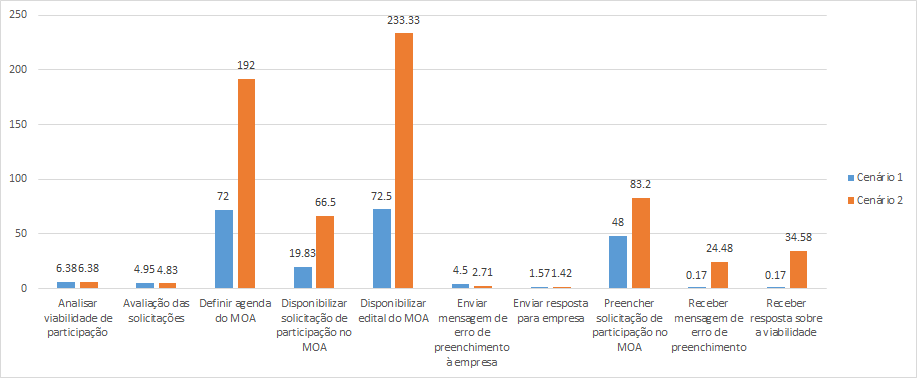
\includegraphics[scale=0.66]{resultado_asis_simulacao}
	\caption[Gráfico de Resultados da Simulação AS-IS]{Gráfico de Resultados da Simulação AS-IS.}
	\label{fig:resultadosasis}
\end{figure}

\subsection[Recursos]{Recursos}
\label{subsec:contexto_asis_recursos}
	\begin{figure}[H]
	\centering
	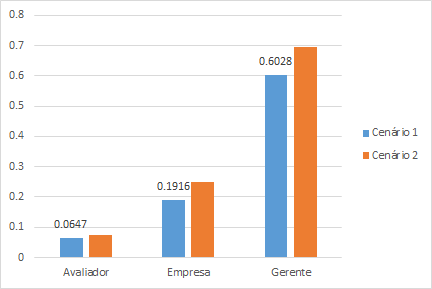
\includegraphics[scale=1]{recursos_asis_simulacao}
	\caption[Gráfico de Recursos da Simulação AS-IS]{Gráfico de Recursos da Simulação AS-IS.}
	\label{fig:recursosasis}
\end{figure}

\subsection[Análise do Resultado]{Análise do Resultado}
\label{subsec:contexto_asis_analise}
	Para ambos os cenários as atividade Definir Agenda do MOA, Disponibilizar Solicitação de Participação no MOA e Disponibilizar Edital do MOA apresentaram um valor mais elevado quanto a média de horas das demais atividades, isso resultou no alto valor para utilização do Gerente no processo.
\\ \indent As demais atividades apresentaram valores próximos do esperado no Cenário 1. No Cenário 2 o tempo foi discrepante devido ao gargalo gerado pelas atividades iniciais do gerente, que acabam influenciando todas as demais. A baixa utilização do analista se mostra preocupante, pois se espera que ele utilize mais o tempo do processo avaliando as solicitações.